{}\documentclass[letterpaper,
compress,
xcolor=x11names,
%draft,
]{beamer}
% Package imports
\usepackage{mathtools} % imports `amsmath'
\DeclareMathOperator{\sech}{sech}
\usepackage{amssymb}
\usepackage{fixltx2e}
\usepackage{lmodern}
\usepackage{movie15}
\usepackage{hyperref}
%\usepackage{media9}
\usepackage{microtype}
\usepackage{animate}
\usepackage{subcaption}
\captionsetup{compatibility=false}

% I just did this
\usepackage[english]{babel}
\usepackage[utf8]{inputenc}
\usepackage{amsmath}
\usepackage{graphicx}
\usepackage[colorinlistoftodos]{todonotes}
\usepackage{tikz}
\usetikzlibrary{tikzmark}
\usepackage{array}
\usepackage{layout}
\usepackage{multicol}
\usepackage{multirow}
\usepackage{booktabs}
%I just did this

% `beamer' configuration
\usefonttheme{professionalfonts}
\useoutertheme[subsection=false,]{miniframes}
\setbeamercolor*{alerted text}{fg=red}
\setbeamercolor*{example text}{fg=black}
\definecolor{CSU_green}{RGB}{30, 70, 43}
\definecolor{CSU_gold}{RGB}{200, 195, 114}
\setbeamercolor*{lower separation line head}{bg=CSU_gold}
\setbeamercolor*{section in head/foot}{fg=white,bg=CSU_green}
\setbeamercolor*{subsection in head/foot}{bg=white}
\setbeamercolor*{upper separation line head}{bg=CSU_gold}
\setbeamercolor*{page number in head/foot}{fg=CSU_green}
\setbeamercolor*{normal text}{fg=black,bg=white}
\setbeamercolor*{palette tertiary}{fg=black,bg=black!10}
\setbeamercolor*{palette quaternary}{fg=black,bg=black!10}
\setbeamercolor*{structure}{fg=black}
\setbeamerfont{frametitle}{shape=\scshape}
\setbeamerfont{institute}{shape=\scshape}
\setbeamerfont{section in head/foot}{shape=\scshape}
\setbeamerfont{subsection in head/foot}{shape=\scshape}
\setbeamertemplate{bibliography item}{}
\setbeamertemplate{itemize items}[ball]
\setbeamertemplate{navigation symbols}{}
\setbeamertemplate{footline}[frame number]
\usetikzlibrary{calc,arrows}
\graphicspath{{graphics/}{graphics/movies/}{graphics/images/}}
\usepackage{remreset}                  % hack to display beamer navigation
\makeatletter                          % circles even if not declaring
\@removefromreset{subsection}{section} % subsections
\makeatother                           % see: http://tex.stackexchange.com/a/2078
\setcounter{subsection}{1}             % see: https://bitbucket.org/rivanvx/beamer/issue/218

% `biblatex' configuration
\usepackage[backend=biber,
style=authortitle-comp,
]{biblatex}
\addbibresource{presentation.bib}

% `enumitem' configuration
\usepackage{enumitem}
\setlist[itemize,1]{label=\usebeamertemplate{itemize item}}
\setlist[itemize,2]{label=\usebeamertemplate{itemize subitem}}
\setlist[itemize,3]{label=\usebeamertemplate{itemize subsubitem}}
\DeclareMathOperator{\sinc}{sinc}


% `graphicx' configuration
\usepackage{graphicx}
\begin{document}
	\title{Course Introduction}
	%\subtitle{MATH-151:  Mathematical Algorithms in Matlab}
	\author{MATH-151:  Mathematical Algorithms in Matlab}
	\date[202X]{August 21, 2023}
	\titlegraphic{
\includegraphics[height = 3cm]{CSU_Ram_Logo.jpg}}



%%%%%%%%%%%%%%%%%%%%%%%%%%%%%%%%%%%%%%%%%%%%%%%%%%%%%%

\begin{frame}
\titlepage
\end{frame}
%%%%%%%%%%%%%%%%%%%%%%%%%%%%%%%%%%%%%%%%%%%%%%%%%%%%%%%%%
\section{About The Class}

\begin{frame}{Algorithms}
	\footnotesize
	\begin{itemize}
		\item Who here would say they think computers are smart?
		\item<2-> At base level, they are actually pretty limited.
		\begin{itemize}
			\item Receive, store, and output data
			\item Add or multiply two numbers
		\end{itemize}
		\item<3-> But they are very good at following directions! By being clever, we can tell the computer to do these operations in very specific ways to achieve bigger goals! These are called algorithms.
		\item<4-> We will use algorithms to make computers do the work for us.
	\end{itemize}
	\onslide<4->{
	\begin{center}
		
\includegraphics[width = 0.5\linewidth]{computer_work.png}
	\end{center}}
\end{frame}
%%%%%%%%%%%%%%%%%%%%%%%%%%%%%%%%%%%%%%%%%%%%%%%%%%%%%%%%%%%%%%%%%%
\begin{frame}{Mathematical Algorithms in Matlab}
	\footnotesize
	\noindent In this course students will be introduced to common algorithms used to numerically solve problems as well as learn how to implement them in the Matlab programming language. \\ 
	\bigskip
	\textcolor{blue}{\href{https://www.mathworks.com/academia/tah-portal/colorado-state-university-40638290.html}{Click here to install Matlab}} \\
	\bigskip
	\noindent Upon completion of this course, the student is expected to have the following skills:
	\begin{itemize}
		\item Ability to write and run common algorithms in Matlab, with coding familiarity transferable to other languages
		\item Effective code commenting and formatting, to ensure code is readable to others
		\item Understanding of algorithm design and how a computer ``thinks"
		\item Debug code to identify and fix mistakes.
	\end{itemize}	
	
\end{frame}

%%%%%%%%%%%%%%%%%%%%%%%%%%%%%%%%%%%%%%%%%%%%%%%%%%%%%%%%%%%%%%%%%%

\begin{frame}{Applications}
	\centering
			$\vcenter{\hbox{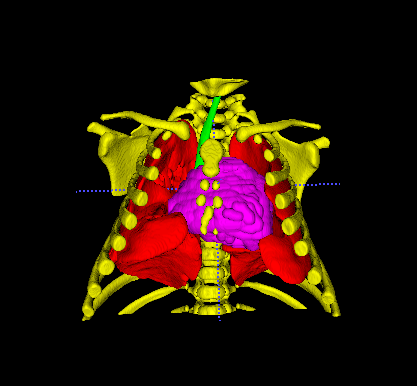
\includegraphics[height = 2.5cm]{ITK_SNAP_3dSeg_case-147596.png}}}$ 
			$\vcenter{\hbox{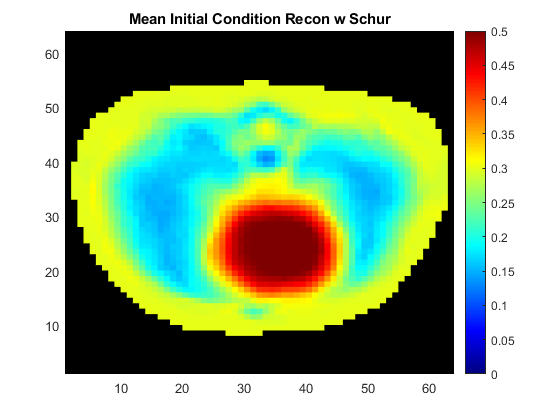
\includegraphics[height = 3cm]{EIT_Recon_Example.png}}} $ \\
			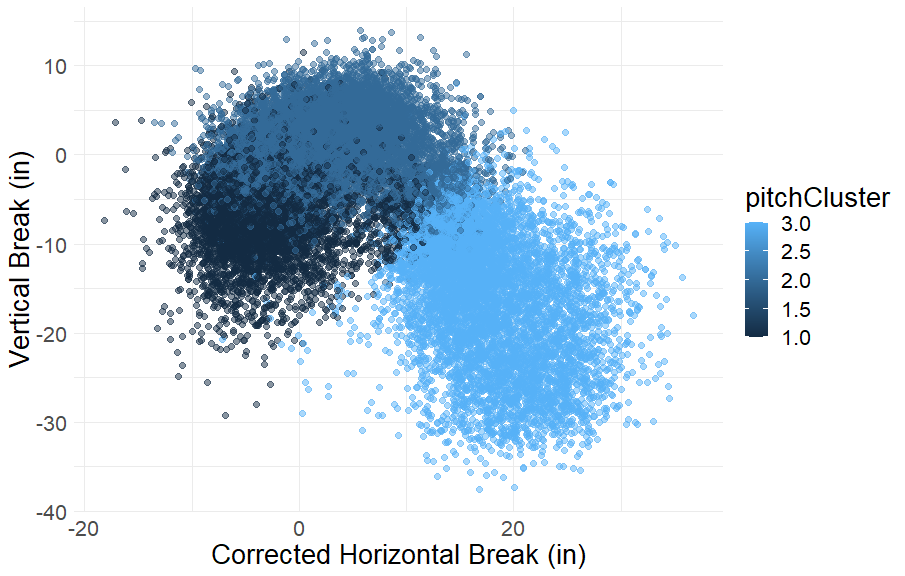
\includegraphics[height = 3cm]{pitchClusters.png} \hfill
			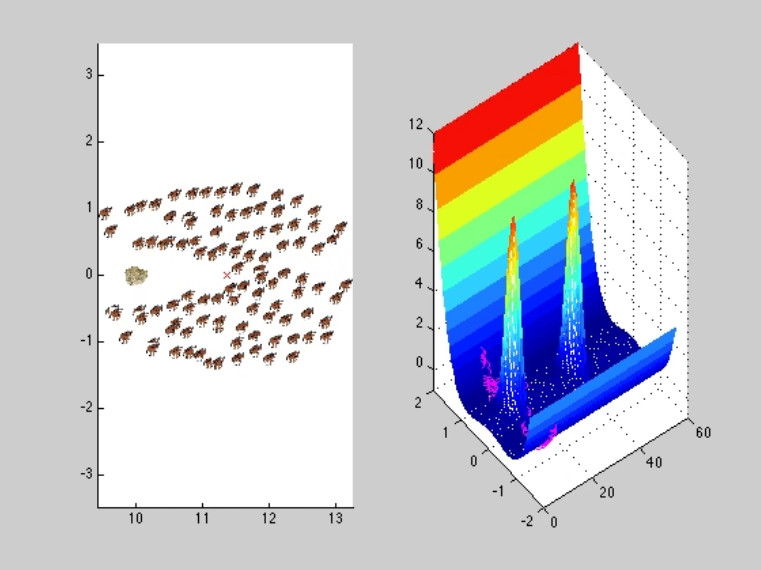
\includegraphics[height = 3cm]{WildBeasts_Still.png}
\end{frame}

%%%%%%%%%%%%%%%%%%%%%%%%%%%%%%%%%%%%%%%%%%%%%%%%%%%%%%%%%%%%%%%%%%
\section{About Me}

\begin{frame}{Who Am I?}
	\begin{itemize}
		\item Education
		\begin{itemize}
			\item PhD Student. Mathematics, CSU, Current
			\item M.S. Applied Mathematics, UMass-Amherst, 2014
			\item B.S. Applied Mathematics, RPI, 2011
		\end{itemize}
		\item Work and Teaching
		\begin{itemize}
			\item Previously worked as a Sr. Systems Engineer
			\item Taught on the side for 4 years
		\end{itemize}
		\item<2-> Interests and Hobbies
		\begin{itemize}
			\item Baseball
			\item Tabletop and video games
			\item<3-> I can go pretty fast on rollerblades ... 
		\end{itemize}
	\end{itemize}
	\begin{center}
		\onslide<2->{
		
\includegraphics[height = 2cm]{ChrisPawSox.jpg}
		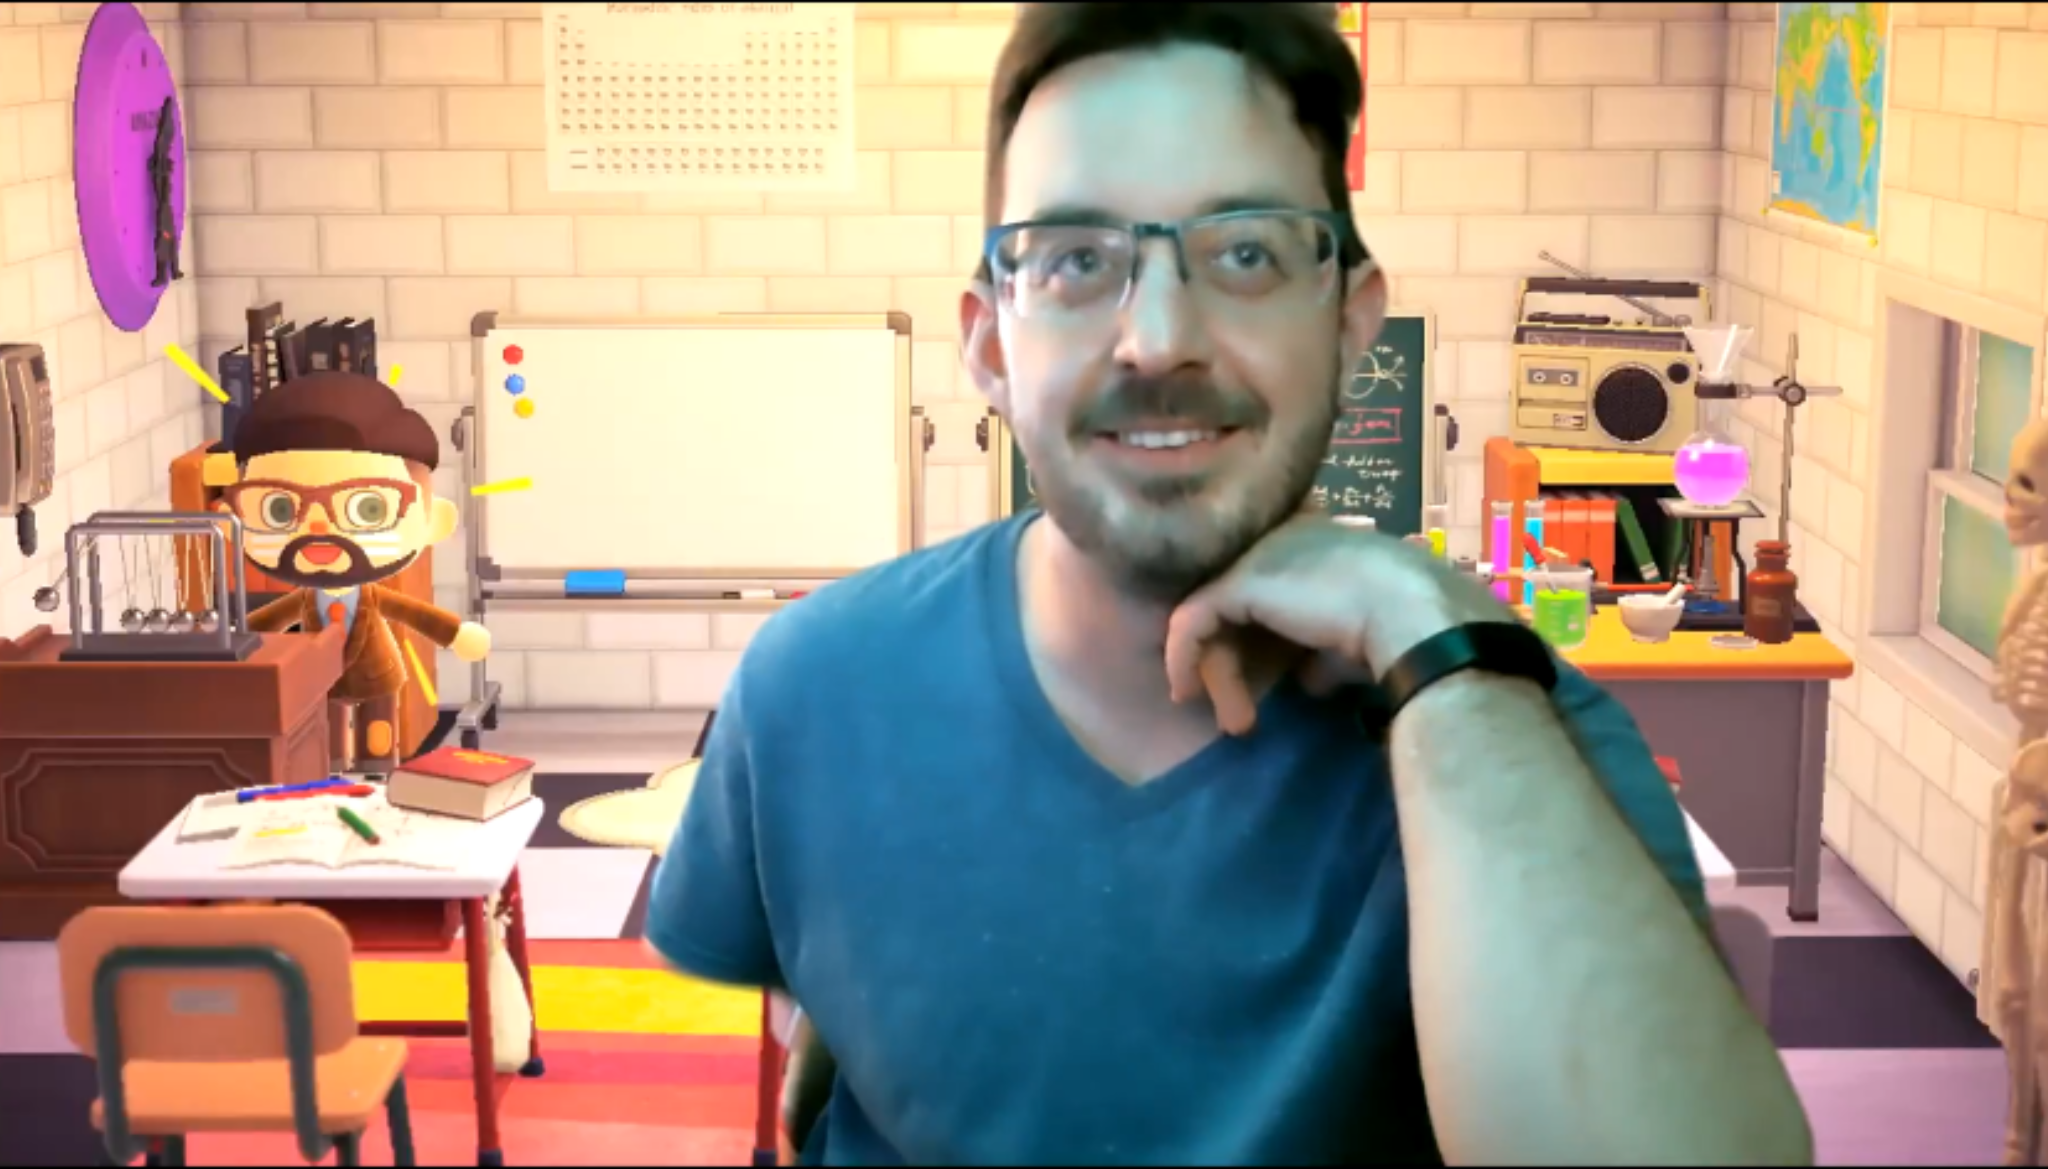
\includegraphics[height = 2cm]{Chris_AC.png}
		
\includegraphics[height = 2cm]{ChrisMii.jpg}
		}
		\onslide<3->{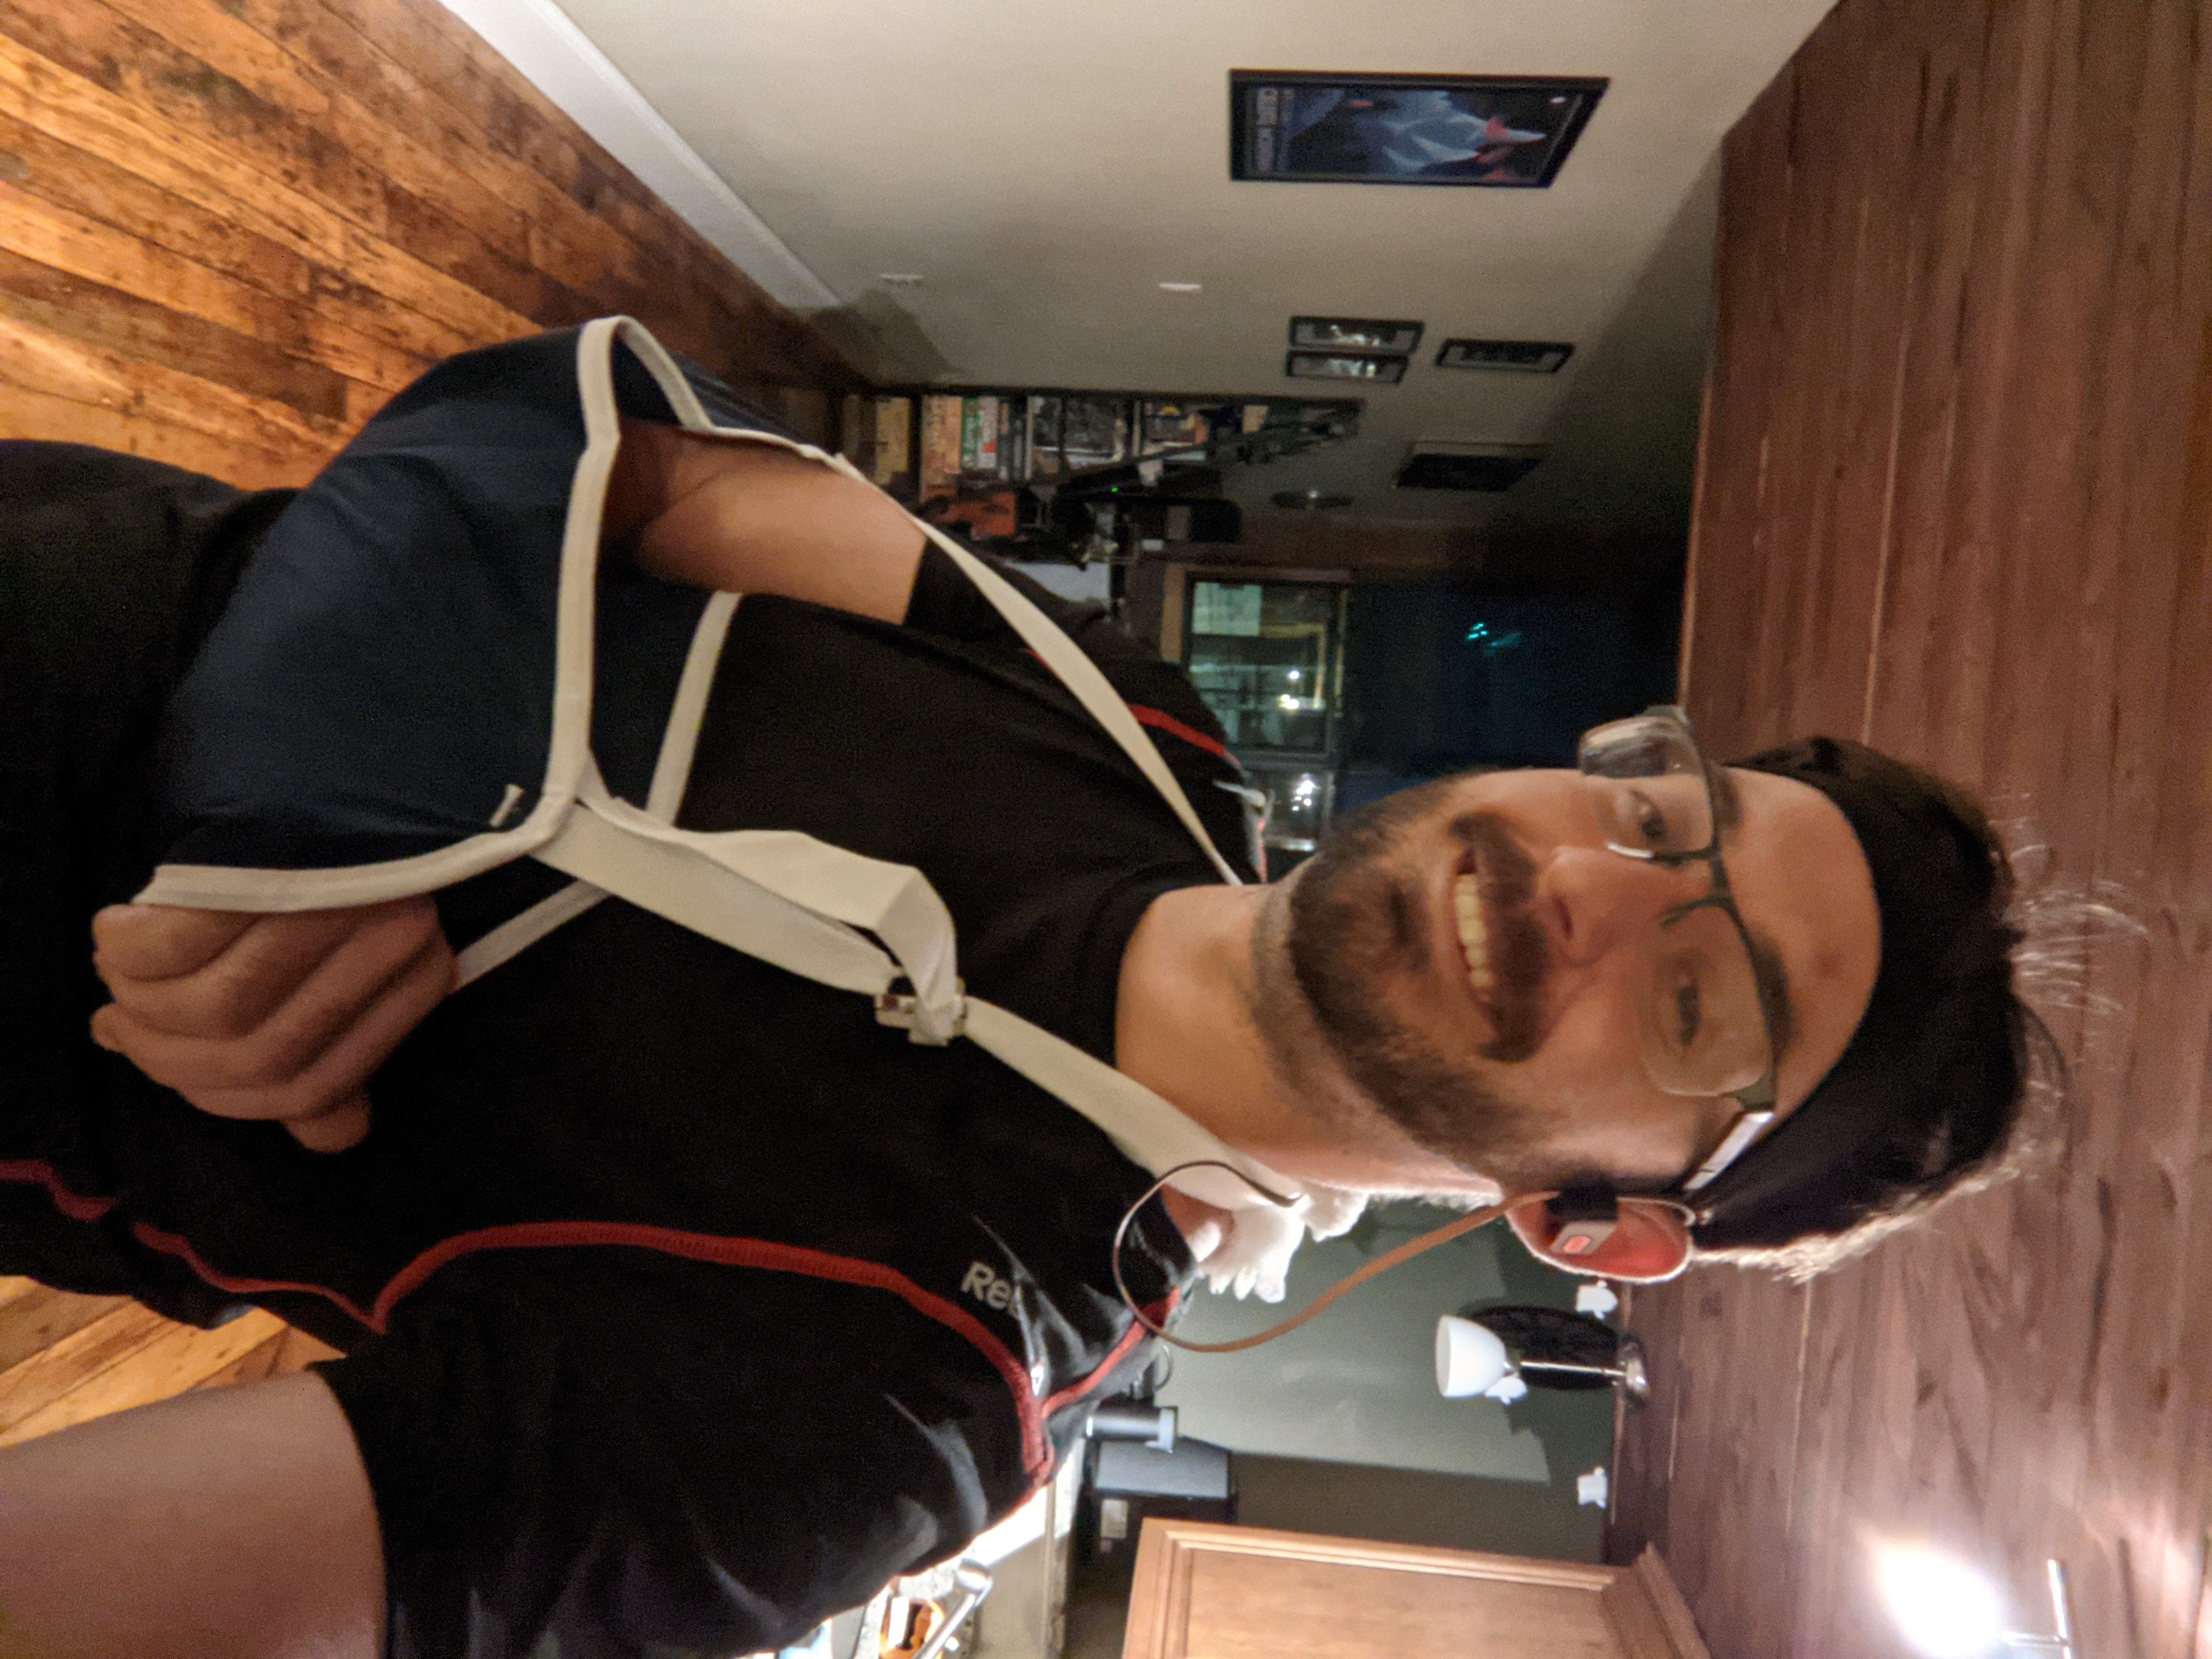
\includegraphics[angle = 90, height = 2cm]{Broken_Chris.jpg}}
	\end{center}
\end{frame}
%%%%%%%%%%%%%%%%%%%%%%%%%%%%%%%%%%%%%%%%%%%%%%%%%%%%%%%%%%
\begin{frame}{My Teaching Philosophy}
	\begin{itemize}
	\item The best I can do as an instructor is to expose the class to course materials and help students gain familiarity with the topics.
	\item Learning occurs when students \textbf{engage with the material}.
	\begin{itemize}
		\item<2-> Actively following along with lectures.
		\begin{itemize}
			\footnotesize
			\item Taking notes.
			\item Thinking about material.
			\item Asking questions.
		\end{itemize}
		\item<3-> Working through problems.
		\begin{itemize}
			\footnotesize
			\item Doing labs with intent. Working in groups is highly recommended.
			\item Understand the purpose of each step.
			\item Discussing approaches and solutions to your peers.
			\item Learn from your mistakes!
		\end{itemize}
	\end{itemize}
	\item<4-> Don't be afraid to talk to me if you are struggling, I am very willing to help!
	\end{itemize}
\end{frame}

\section{Course Syllabus}
%%%%%%%%%%%%%%%%%%%%%%%%%%%%%%%%%%%%%%%%%%%%%%%%%%%%%%%%%
\begin{frame}{Course Grading Scheme}
	\footnotesize
	\begin{itemize}
		\item\textbf{Lecture Journals (\underline{5\%})}
			\begin{itemize}
				\item Short writing prompt assigned about each lecture
				\item Graded based on completion
			\end{itemize}
		\item<2->\textbf{Labs (\underline{80\%})}
			\begin{itemize}
				\item Hands-on coding problems assigned each week
				\item Due before Monday class the following week.
			\end{itemize}
		\item<3->\textbf{Final Lab (\underline{15\%})}
			\begin{itemize}
				\item Cumulative lab assignment connecting various algorithms seen in class
			\end{itemize}
		\item<4-> Lab grading will be based on the ``three C's", 
			\begin{itemize}
				\item \textbf{C}ompletion: Is the lab completed?
				\item \textbf{C}orrectness: Does the code perform as desired?
				\item \textbf{C}larity: Is the code well presented? Is the code commented?
			\end{itemize}
	\end{itemize}
\end{frame}
%%%%%%%%%%%%%%%%%%%%%%%%%%%%%%%%%%%%%%%%%%%%%%%%%%%%%%%%%
\begin{frame}{Tentative Schedule}
	\tiny
	
	\begin{center}
		\begin{tabular}{l || l | l | l }
			\toprule
			\textbf{Dates} & \textbf{Monday} & \textbf{Wednesday} & \textbf{Friday}\\
			\midrule
			8/21  - 8/25  & Course Introduction           & General Coding Concepts & Matlab Introduction  \\
			8/28  - 9/1   & Logic and Loops               & Lab 1                   & Extra Lab Time       \\
			9/4   - 9/8   & \textbf{No Class!}            & Vectors and Plotting    & Lab 2                \\
			9/11  - 9/15  & Functions and Recursion       & Lab 3                   & Extra Lab Time       \\
			9/18  - 9/22  & Interpolation                 & Lab 4                   & Extra Lab Time       \\
			9/25  - 9/29  & Numerical Integration         & Lab 5                   & Extra Lab Time       \\
			10/2  - 10/6  & Numerical Differentiation     & Lab 6                   & Extra Lab Time       \\
			10/9  - 10/13 & Nonlinear Solvers             & Lab 7                   & Extra Lab Time       \\
			10/16 - 10/20 & Differential Equation Solvers & Lab 8                   & Extra Lab Time       \\
			10/23 - 10/27 & Final Exam                    & Final Exam              & Final Exam           \\
			\bottomrule
			\multicolumn{4}{l}{$^{*}$ Schedule subject to change as necessary.}\\
		\end{tabular}
	\end{center}
\end{frame}
%%%%%%%%%%%%%%%%%%%%%%%%%%%%%%%%%%%%%%%%%%%%%%%%%%%%%%%%%
\end{document}